%
% This is a borrowed LaTeX template file for lecture notes for CS267,
% Applications of Parallel Computing, UC Berkeley EECS Department.
% Now being used for Carnegie Mellon University's 10-725/36-725 
% Convex Optimization course taught by Ryan Tibshirani.  When
% preparing LaTeX notes for this class, please use this template. 
%
% To familiarize yourself with this template, the body contains
% some examples of its use.  Look them over.  Then you can
% run LaTeX on this file.  After you have LaTeXed this file then
% you can look over the result either by printing it out with
% dvips or using xdvi. "pdflatex template.tex" should also work.
%

\documentclass[twoside]{article}
\setlength{\oddsidemargin}{0.25 in}
\setlength{\evensidemargin}{-0.25 in}
\setlength{\topmargin}{-0.6 in}
\setlength{\textwidth}{6.5 in}
\setlength{\textheight}{8.5 in}
\setlength{\headsep}{0.75 in}
\setlength{\parindent}{0 in}
\setlength{\parskip}{0.1 in}

%
% ADD PACKAGES here:
%

\usepackage{amsmath,amsfonts,graphicx}
\usepackage{amsmath,textcomp,amssymb,geometry,graphicx,hyperref,mathtools,textcomp}
\usepackage[final]{pdfpages}
\usepackage[export]{adjustbox}
\usepackage{enumerate}
\usepackage{titlesec}
\usepackage{listings}
%\usepackage[usenames, dvipsnames]{color}
\usepackage{cleveref}



%\DeclarePairedDelimiter\ceil{\lceil}{\rceil}%
%\DeclarePairedDelimiter\floor{\lfloor}{\rfloor}%
%\DeclarePairedDelimiter\abs{\lvert}{\rvert}%
%\DeclarePairedDelimiter\norm{\lVert}{\rVert}%
%\newcommand{\E}{\mathbb{E}}
\newcommand{\R}{\mathbb{R}}
\newcommand{\st}{\text{s.t.}}
\newcommand{\Var}{\mathrm{Var}}
% From http://tex.stackexchange.com/questions/79434/
\newcommand\independent{\protect\mathpalette{\protect\independenthelper}{\perp}}
%\def\independenthelper#1#2{\mathrel{\rlap{$#1#2$}\mkern2mu{#1#2}}}


%
% The following commands set up the lecnum (lecture number)
% counter and make various numbering schemes work relative
% to the lecture number.
%
\newcounter{lecnum}
\renewcommand{\thepage}{\thelecnum-\arabic{page}}
\renewcommand{\thesection}{\thelecnum.\arabic{section}}
\renewcommand{\theequation}{\thelecnum.\arabic{equation}}
\renewcommand{\thefigure}{\thelecnum.\arabic{figure}}
\renewcommand{\thetable}{\thelecnum.\arabic{table}}

%
% The following macro is used to generate the header.
%
\newcommand{\lecture}[4]{
   \pagestyle{myheadings}
   \thispagestyle{plain}
   \newpage
   \setcounter{lecnum}{#1}
   \setcounter{page}{1}
   \noindent
   \begin{center}
   \framebox{
      \vbox{\vspace{2mm}
    \hbox to 6.28in { {\bf 10-725/36-725: Convex 
        Optimization \hfill Fall 2015} }
       \vspace{4mm}
       \hbox to 6.28in { {\Large \hfill Lecture #1: #2  \hfill} }
       \vspace{2mm}
       \hbox to 6.28in { {\it Lecturer: #3 \hfill Scribes: #4} }
      \vspace{2mm}}
   }
   \end{center}
   \markboth{Lecture #1: #2}{Lecture #1: #2}

   {\bf Note}: {\it LaTeX template courtesy of UC Berkeley EECS dept.}

   {\bf Disclaimer}: {\it These notes have not been subjected to the
   usual scrutiny reserved for formal publications. They may be
   distributed outside this class only with the permission of the
   Instructor.} \vspace*{4mm}
}


%
% Convention for citations is authors' initials followed by the year.
% For example, to cite a paper by Leighton and Maggs you would type
% \cite{LM89}, and to cite a paper by Strassen you would type \cite{S69}.
% (To avoid bibliography problems, for now we redefine the \cite command.)
% Also commands that create a suitable format for the reference list.
\renewcommand{\cite}[1]{[#1]}
\def\beginrefs{\begin{list}%
        {[\arabic{equation}]}{\usecounter{equation}
         \setlength{\leftmargin}{2.0truecm}\setlength{\labelsep}{0.4truecm}%
         \setlength{\labelwidth}{1.6truecm}}}
\def\endrefs{\end{list}}
\def\bibentry#1{\item[\hbox{[#1]}]}

%Use this command for a figure; it puts a figure in wherever you want it.
%usage: \fig{NUMBER}{SPACE-IN-INCHES}{CAPTION}
\newcommand{\fig}[3]{
			\vspace{#2}
			\begin{center}
			Figure \thelecnum.#1:~#3
			\end{center}
	}
% Use these for theorems, lemmas, proofs, etc.
\newtheorem{theorem}{Theorem}[lecnum]
\newtheorem{lemma}[theorem]{Lemma}
\newtheorem{proposition}[theorem]{Proposition}
\newtheorem{claim}[theorem]{Claim}
\newtheorem{corollary}[theorem]{Corollary}
\newtheorem{definition}[theorem]{Definition}
\newenvironment{proof}{{\bf Proof:}}{\hfill\rule{2mm}{2mm}}

% **** IF YOU WANT TO DEFINE ADDITIONAL MACROS FOR YOURSELF, PUT THEM HERE:

\newcommand\E{\mathbb{E}}

\begin{document}
%FILL IN THE RIGHT INFO.
%\lecture{**LECTURE-NUMBER**}{**DATE**}{**LECTURER**}{**SCRIBE**}
\lecture{11}{October 5}{Ryan Tibshirani}{Achal Dave, Anirudh Vemula, Vishal Dugar}
%\footnotetext{These notes are partially based on those of Nigel Mansell.}

% **** YOUR NOTES GO HERE:

% Some general latex examples and examples making use of the
% macros follow.  
%**** IN GENERAL, BE BRIEF. LONG SCRIBE NOTES, NO MATTER HOW WELL WRITTEN,
%**** ARE NEVER READ BY ANYBODY.

%\section{Last Class: Duality in Linear Programs}

%In last class, we discussed two explanations for how we formulate the dual problem in linear programs.\\
%\textit{Explanation \#1}: We multiply the corresponding dual variables to each of the constraints in the primal problem and sum the expressions. This gives us an expression similar to the primal criterion which is lower bounded. Equating this expression to the primal criterion, we get equality constraints, in addition to the inequality constraints obtained by introducing the dual variables. \\
%\textit{Explanation \#2}: Alternatively, we can construct the Lagrangian by introducing a dual variable for each constraint, multiplying it with the constraint and adding it to the criterion. We can observe that the Lagrangian (constructed this way) is a lower bound on the primal criterion, for any value of the dual variables. This method reproduces the same dual as \#1 above, but is actually completely general and applies to arbitrary optimization problems (even non-convex programs and not just linear programs)


\section{Lagrangian}

Consider any general minimization problem
\begin{alignat*}{2}
&\min_x &&f(x) \\
&\text{ subject to}&~&h_i(x) \leq 0, i = 1, \dots, m \\
&&&l_j(x) = 0, j = 1, \dots, r
\end{alignat*}

Let's define the Lagrangian, introducing variables $u \in \R^m, v \in \R^r$,
with $u \geq 0$.
\begin{align*}
L(x, u, v) = f(x) + \sum_{i=1}^m u_i h_i(x) + \sum_{j=1}^r v_j l_j(x)
\end{align*}

It turns out that for any $u \geq 0$ and any $v$, we have that
\begin{align*}
L(x, u, v) = f(x) \sum_{i=1}^m u_i \underbrace{h_i(x)}_{\leq 0} + \sum_{j=1}^r v_j \underbrace{l_j(x)}_{=0} \leq f(x)
\end{align*}
Thus, we can observe that the Lagrangian $L(x, u, v)$ is always a lower bound for the primal criterion $f(x)$ for any value of $u \geq 0$ and $v$. An example for this is shown in the figure below:

\begin{figure}[h]
  \centering
  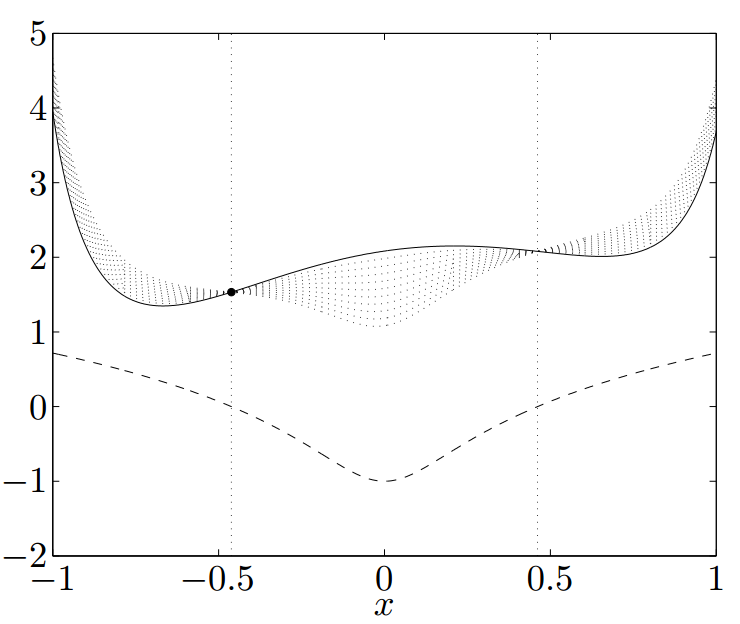
\includegraphics[scale=0.3]{lagrangian.png}
  \caption{Solid line is $f$, dashed line is $h$. Each dotted line shows $L(x,u,v)$ for different choices of $u \geq 0$ and $v$. Note that the feasible set is $x \in [-0.46, 0.46]$}
  \label{fig:lagrangian}
\end{figure}

And so, we have that if $f^*$ be the primal optimal value and $C$ is the primal
feasible set, then
\begin{align*}
f^* \geq \min_{x \in C} L(x, u, v) \geq \min_x L(x, u, v) \triangleq g(u, v)
\end{align*}

This $g(u, v)$ is the \textbf{Lagrange dual function}, and it provides a lower
bound on the optimal value $f^*$ for any dual feasible $u, v$ (i.e. $u \geq 0$
and any $v$).

Generally, duality will provide us with a tight lower bound in the
\textit{convex} case, but this need not be the true in the \textit{non-convex} case. One such example is shown in the figure below, where the lower bound is not tight:
\begin{figure}[h]
  \centering
  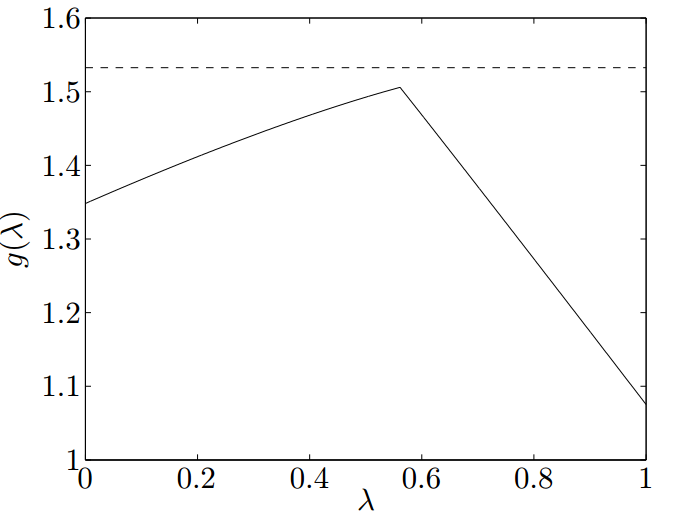
\includegraphics[scale=0.3]{tightness.png}
  \caption{Dashed horizontal line is $f^*$, dual variable is $\lambda$ and solid line shows $g(\lambda)$}
  \label{fig:tightness}
\end{figure}

\subsection{Example: Quadratic Program}
Consider a quadratic program where $Q \succ 0$:
\begin{alignat*}{2}
&\min_x& &\frac{1}{2} x^T Q x + c^T x \\
&\text{ subject to}&~&Ax = b, x \geq 0
\end{alignat*}

In this case, our Lagrangian is simply
\[ L(x, u, v) = \frac{1}{2} x^T Q x + c^T x - u^T x + v^T(Ax - b) \]

To compute the dual function $g(u, v) = \min_x L(x, u, v)$, we minimize the
Lagrangian above by taking the gradient with respect to $x$ and setting it equal
to zero, and we get that
\begin{align*}
x^* &= -Q^{-1}(c - u + A^T v) \\
\implies \min_x L(x, u, v) &= L(x^*, u, v) \\
    &= \frac{1}{2} (c - u + A^T v)^T Q^{-1}(c - u + A^T v) - (c - u + A^T v)^T Q^{-1}(c - u + A^T v) - b^T v \\
    &= -\frac{1}{2} (c - u + A^T v)^T Q^{-1}(c - u + A^T v) - b^T v
\end{align*}

What if, instead, we had the same QP as above, except $Q
\mathbin{\textcolor{red}{\succeq}} 0$ (i.e. Q is only positive
\textit{semi}-definite).  Then, if we try to minimize the Lagrangian above by
setting the gradient to 0, we get the following constraint at the optimum:
\begin{align}
Qx = -(c - u + A^T v) \label{eq:qp_semidefinite_zero_gradient}
\end{align}

Now, there are two cases:
\begin{enumerate}[(i)]
\item $c - u + A^T v \in \text{col}(Q)$. Then, we can use the pseudo-inverse (see below)
      $Q^{\dagger}$ of $Q$. This also implies that $P \left( c - u + A^T v \right) = 0$, where $P$ is the projection matrix onto $\text{null}\left(Q\right)$.
\item $c - u + A^T v \not\in \text{col}(Q)$, which implies that $c - u + A^T v$
      is not orthogonal to the null space of $Q$. Then, let
      \[ c - u + A^T v = z_1 + z_2, \]
      where $z_1 \in \text{col}(Q), z_2 \in \text{null}(Q), z_2 \neq 0$. But
      in this case, there is no $x$ that satisfies
      \cref{eq:qp_semidefinite_zero_gradient}, and so there is no unique
      minimizer $x^*$. But $L(x, u, v)$ is quadratic in $x$, so if there is no
      minimizer of $L(x, u, v)$ in $x$, the minimum must be $L(x, u, v) =
      -\infty$.
\end{enumerate}

So,
\begin{align*}
g(u, v) = \begin{cases}
-\frac{1}{2} (c - u + A^T v)^T Q^{\dagger} (c - u + A^Tv) - b^T v ~&\text{case (i)} \\
-\infty ~&\text{case (ii)}
\end{cases}
\end{align*}

\subsubsection{Aside: Pseudo-inverse}
For a general matrix $A \in \R^{n\times n}$, we can define the pseudo-inverse
$A^{\dagger}$ in terms of its Singular Vector Decomposition. Using SVD, we can
write $A$ as
\[ A = U D V^T \]

If $A$ was invertible, we can directly invert the decomposition above:
\[ A^{-1} = (U D V^T)^{-1} = (V^T)^{-1} D^{-1} U^{-1} = V D^{-1} U^T \]
where
\begin{align*}
D^{-1} = \begin{bmatrix}
\frac{1}{d_1} & 0 & \dots & 0 \\
0 & \frac{1}{d_2} & \dots & 0 \\
0 & 0 & \ddots & \vdots \\
0 & 0 & \dots & \frac{1}{d_n} \\
\end{bmatrix}
\end{align*}

If $A$ is not invertible, we're going to see that for $k = \text{rank}(A)$,
$d_{k+1} = d_{k+2} = \dots = d_n = 0$. In this case, we can construct
a pseudo-inverse ($D^{\dagger}$) of $D$ as follows:
\begin{align*}
D^{\dagger} = \begin{bmatrix}
\frac{1}{d_1} & 0 & \dots & 0 & 0  & 0 & 0\\
0 & \frac{1}{d_2} & \dots & 0 & 0  & 0 & 0\\
0 & 0 & \ddots & \vdots & 0  & 0 & 0\\
0 & 0 & \dots & \frac{1}{d_k} & 0  & 0 & 0\\
0 & 0 & \dots & 0 & 0  & 0 & 0\\
0 & 0 & \dots & 0 & 0  & \ddots & 0\\
0 & 0 & \dots & 0 & 0  & 0 & 0\\
\end{bmatrix}
\end{align*}

And our pseudo-inverse, then, is
\begin{align*}
A^{\dagger} = V D^{\dagger} U^T
\end{align*}

\subsection{Example: Quadratic Program in 2D}
\label{sec:exampl-quadr-progr}

In this example, we choose $f(x)$ to be quadratic in 2 variables, subject to $ x \geq 0$. The dual function $g(u)$ is also quadratic in 2 variables, also subject to $u \geq 0$. In the figure below, we can see that the dual function $g(u)$ provides a bound on $f^*$ for every $u \geq 0$, and the largest bound $g(u)$ gives us turns out to be exactly $f^*$! In the future, we will see that this is not a coincidence and results from KKT conditions.

\begin{figure}[h]
  \centering
  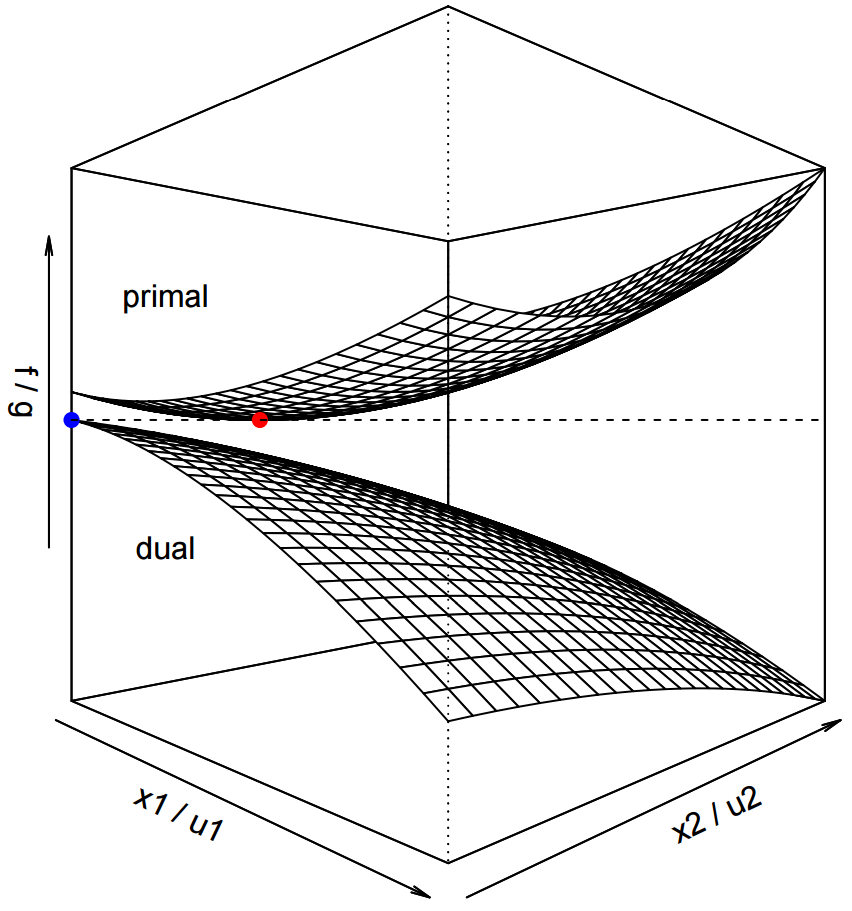
\includegraphics[scale=0.3]{quad.png}
  \caption{Blue dot is the optimal dual value and the red dot is the optimal primal value}
  \label{fig:quad}
\end{figure}

\section{Lagrange Dual Problem}
\label{sec:lagr-dual-probl}
Given the primal problem
\begin{alignat*}{3}
&\min_x &&f(x) \\
&\text{subject to } && h_i(x) \leq 0 ~~~&&\text{for } 1 \leq i \leq m \\
&&& l_j(x) = 0 ~~~&&\text{for } 1 \leq j \leq r
\end{alignat*}

We have shown that our constructed dual function $g(u,v)$ satisfies the property $f^* \geq g(u,v)$ for all $u \geq 0$ and $v$. Thus, we get the tightest lower bound on the optimal primal criterion $f^*$ by maximizing $g(u,v)$ over all dual feasible $u,v$, yielding the Lagrange dual problem:
\begin{alignat*}{2}
&\max_{u,v} &&g(u,v) \\
&\text{ subject to}&~&u \geq 0 
\end{alignat*}

Note that, if the dual optimal value is $g^*$, then
$$ f^* \geq g^* $$
This always holds (even if the primal problem is nonconvex) and is called the \textit{weak duality} property. 

\subsection{Convexity of the dual}

A very interesting property is that the dual problem is a convex optimization problem (even if the primal problem is non-convex) problem in $u, v$:
\begin{align*}
g(u, v) &= \min_x \{f(x) + \sum_{i=1}^m u_i h_i(x) + \sum_{j=1}^r v_j l_j(x) \} \\
        &= - \underbrace{\max_x \{-f(x) - \sum_{i=1}^m u_i h_i(x) - \sum_{j=1}^r v_j l_j(x) \}}_{\text{pointwise maximum of convex functions in } (u, v)}
\end{align*}
As can be observed from above, $g(u,v)$ can be expressed as the negative of pointwise maximum of convex functions in $(u,v)$. Hence, $g$ is concave in $(u,v)$, and $u \geq 0$ is a convex constraint, hence the dual problem is a concave maximization problem (or a convex minimization problem if we consider $-g$)


So why don't we just always write down the dual problem and solve it, if it's
convex? It turns out computing $g(u, v)$ is hard in and of itself, since it
involves a maximization over $x$, especially for non-convex problems. In other
words, we might not be able to write out $g(u, v)$ in the first place!

\section{Strong Duality}
We know that $f^* \geq g^*$, which is known as weak duality. In some problems, we
see that $f^* = g^*$. This is known as \textbf{strong duality}.

\textbf{Slater's condition}: If the primal is a convex problem, and there exists
at least one \textit{strictly} feasible $x \in \R^n$, then strong duality holds.

That is, for a general convex primal problem,
\begin{alignat*}{3}
&\min_x &&f(x) \\
&\text{subject to } && h_i(x) \leq 0 ~~~&&\text{for } 1 \leq i \leq m \\
&&& l_j(x) = 0 ~~~&&\text{for } 1 \leq j \leq r
\end{alignat*}

where $h_i(x)$ is convex and $l_j(x)$ is affine, and a strictly feasible $x$ is
an $x$ such that for every $i, h_i(x) < 0$ and for every
$j, l_j(x) = 0$. This is a weak condition, and an important extension to Slater's condition maintains that strict inequalities \emph{only} need to hold over $h_i\left(x\right)$ that are \emph{not affine}.

\subsection{Strong duality for Linear Programs}
For linear programs
\begin{itemize}
\item The dual of the dual is the primal.
\item Strong duality holds for the primal LP if it is feasible (refinement over Slater's conditions).
\item Similarly, strong duality holds for the dual if it is feasible.
\item Thus, strong duality holds for LPs, except when both primal and dual are infeasible.
\end{itemize}

\subsection{Example: SVM dual}
The SVM problem is as follows:
\begin{alignat*}{2}
&\min_{\beta, \beta_{0}, \xi} && \frac{1}{2} \| \beta \|^{2}_{2} + C \sum_{i=1}^{n}\xi_{i} \\
&\text{ subject to}&~& \xi_{i} \geq 0, i = 1, \dots, n \\
&&& y_{i}\left( x_{i}^{T} \beta + \beta_{0} \right) \geq 1-\xi_{i}, i = 1, \dots, n
\end{alignat*}

We form the following Lagrangian with the dual variables $v,w \geq 0$:
\begin{align*}
L\left(\beta, \beta_{0}, \xi, v, w\right) = \frac{1}{2} \| \beta \|^{2}_{2} + C \sum_{i=1}^{n}\xi_{i} - \sum_{i=1}^{n}v_{i}\xi_{i} + \sum_{i=1}^{n} w_{i}\left(1 - \xi_{i} - y_{i}\left(x_{i}^{T}\beta + \beta_{0}\right) \right)
\end{align*}

Minimizing over $\beta, \beta_{0}, \xi$ gives the Lagrange dual:
\begin{align*}
g(v, w) = \begin{cases}
-\frac{1}{2} w^{T}\tilde{X}\tilde{X}^{T}w + 1^{T}w ~& \text{if}\;\; w=C1-v, w^{T}y=0 \\
-\infty ~&\text{otherwise}
\end{cases}
\end{align*}
where $\tilde{X} = \text{diag}\left(y\right)X$. The SVM dual problem can thus be written as:
\begin{alignat*}{2}
&\max_{w} && -\frac{1}{2} w^{T}\tilde{X}\tilde{X}^{T}w + 1^{T}w \\
&\text{ subject to}&~& 0 \leq w \leq C1,\;\; w^{T}y=0 \\
\end{alignat*}

Since $w=0$ is a feasible solution, Slater's conditions are satisfied and we have strong duality.

\section{Duality Gap}
The duality gap $f\left(x\right) - g\left(u,v\right)$ refers to the difference between the primal ($f$) and dual ($g$) criterion values for corresponding $x, u, v$. An important property of the duality gap is the following:
\begin{align*}
f\left(x\right) - f^{*} \leq f\left(x\right) - g\left(u,v\right)
\end{align*}
This implies that a zero duality gap indicates an optimal value for both the primal and the dual. In practice, this provides a stopping criterion; if $f\left(x\right) - g\left(u,v\right) \leq \epsilon$, then $f\left(x\right) - f^{*} \leq \epsilon$.


% **** THIS ENDS THE EXAMPLES. DON'T DELETE THE FOLLOWING LINE:

\end{document}



%%% Local Variables:
%%% mode: latex
%%% TeX-master: t
%%% End:
